\documentclass[a4paper,12pt,oneside]{article}


\usepackage[english]{babel}
\usepackage{caption}
\usepackage[T1]{fontenc}
\usepackage[utf8]{inputenc}
\usepackage{fancyhdr}
\usepackage{lscape}

\usepackage{lmodern}

\usepackage[normalem]{ulem}
\usepackage[left=3cm,right=2cm,top=1.5cm,bottom=1cm,
includeheadfoot,headsep=1cm,
footskip=1cm,headheight=14.599pt]{geometry}

\usepackage[backend=biber, style=apa]{biblatex}
\usepackage{graphicx} 
\usepackage{epstopdf}

\usepackage{tabularx}
\usepackage{longtable}
\usepackage{multirow}

\usepackage{subcaption}

\usepackage{csquotes}


\usepackage{amsmath}
\usepackage{amsthm}
\usepackage{amsfonts}

\usepackage{setspace}
\onehalfspacing

\usepackage{tikz}

\usepackage{adjustbox}
\usepackage{float}

\usepackage{tcolorbox}
\tcbset{colback=white,colframe=orange,
        fonttitle=\bfseries}

\usepackage[colorlinks,pdfpagelabels,pdfstartview=FitH,
bookmarksopen=true,bookmarksnumbered=true,linkcolor=black,
plainpages=false,hypertexnames=false,citecolor=black]{hyperref}


\usepackage{listings}
\usepackage{xcolor}

\usepackage[skip=12pt, indent=0pt, parfill=50pt]{parskip}

\definecolor{codegreen}{rgb}{0,0.5,0} % Slightly darker green for comments
\definecolor{codegray}{rgb}{0.4,0.4,0.4} % Darker gray for line numbers
\definecolor{codepurple}{rgb}{0.5,0,0.5} % A more subdued purple for strings
\definecolor{backcolour}{rgb}{0.98,0.98,0.98} % A lighter background for better contrast

\lstdefinestyle{codeStyle}{
    backgroundcolor=\color{backcolour},   
    commentstyle=\color{codegreen},
    keywordstyle=\color{magenta},
    numberstyle=\tiny\color{codegray},
    stringstyle=\color{codepurple},
    basicstyle=\ttfamily\footnotesize,
    breakatwhitespace=false,         
    breaklines=true,                 
    captionpos=b,                    
    keepspaces=true,                 
    numbers=left,                    
    numbersep=5pt,                  
    showspaces=false,                
    showstringspaces=false,
    showtabs=false,                  
    tabsize=2
}
\lstset{style=codeStyle}

\addbibresource{bib/literature.bib, bib/sites.bib}

\renewcommand{\thesubfigure}{\arabic{subfigure}}

%%%%%%%%%%%%%%%%%%%%%%%%%%%%%%%%%%%%%%%%%%%%%
%% DOCUMENT                                %%
%%%%%%%%%%%%%%%%%%%%%%%%%%%%%%%%%%%%%%%%%%%%%
\begin{document}
    \pagenumbering{gobble}
    

    \pagestyle{empty}
    \begin{titlepage}
    \begin{figure}[!ht]
        % \flushleft
            
\includegraphics[width=0.26\textwidth]{sources/logo_TH-Koeln_CMYK_22pt.eps}
    \end{figure}

    \begin{center}
      \Large
      Cologne University of Applied Sciences\\
      Faculty of Computer Science and Engineering Science\\
      \vspace{0.5cm}
      \hrule\par\rule{0pt}{2cm}
      \LARGE
      \textsc{M A S T E R  T H E S I S}\\
      \vspace{1cm}
      \huge
      Texture Asset generation through Transformer Models\\
      \vspace{1.5cm}
      \large
      Cologne University of Applied Sciences\\
      Campus Gummersbach\\
      Master Digital Sciences\\ 
      \vspace{1.0cm}
      written by:\\
      \textsc{Dennis Goßler}\\
      11140150\\
      \vspace{1.5cm}
      \begin{tabular}{ll}
          \textbf{First examiner:} & Prof. Dr. Olaf Mersmann \\
          \textbf{Second examiner:} & Prof. Dr. Boris Naujoks \\
      \end{tabular}
    
    \end{center}    
    \end{titlepage}
    
    \newpage
    
    
    \begin{abstract}
    TODO
    \end{abstract}
    
    \newpage
    

    \tableofcontents
    
    \newpage
    \pagestyle{fancy}
    
    
    \addcontentsline{toc}{section}{List of Figures}
    \listoffigures
    \newpage
    
    \addcontentsline{toc}{section}{List of tables}
    \listoftables
    \newpage
    
  
    \pagenumbering{arabic}
    
    \section{Introduction}\label{introduction}  
    
In this thesis, we will investigate the use of a traditional Transformer model to generate texture assets to use as floor texture in e.g. in video games. Transformers are usually used to ... . But in this thesis, the focus is to use them to generate the next Pixel in a texture. Multiple different datasets of textures will be used from the internet to train the model. The final developed models will be trained on a GPU cluster in Berlin. The models will be evaluated on a set of metrics and the results will be compared to other models.

\subsection{Related work}
    
\subsection{Data}
    
This section describes the methods used for gathering, cleaning, and analyzing data in a research thesis on textures. Essential for training a machine learning model, the data is carefully collected from various sources, cleaned to maintain uniformity, and examined for patterns, with a focus on color distribution.


\subsubsection{Data Retrieval}
On the internet, a wide variety of textures can be found, but not all of them are suitable for this task. The textures should be seamless, devoid of shadows, and free from any objects. Textures of floors, such as carpets, tiles, wood, concrete, and more, were utilized. Two approaches were employed to acquire the data for this thesis.

\begin{itemize}
    \item Web Data Collection

    The data for this project was obtained from various online sources. Numerous free texture providers, such as textures.com, texturehaven.com, and others, were utilized for data acquisition. Due to the limitation of downloading one texture at a time from most websites, a series of scripts were developed to compile a list of suitable textures and automate the downloading process. These scripts were created using UiPath and Python.
    
    \item Video Game Textures
    
    The second approach involved using textures from video games. The advantage of this approach is that these textures are already seamless and often of high quality and quantity. However, a drawback is that these textures can be very repetitive. To obtain these textures, downward-facing recordings of the game were made, and the textures were extracted from the video. The major challenge with this approach is the need to disable shadows and all UI elements (HUD elements) in the game, which is not always possible.
\end{itemize}

\subsubsection{Data Cleaning}

    To ensure that the data is consistent and free from elements that could corrupt the model, various cleaning steps were applied. For example, all images containing 3D objects were removed, especially those gathered from video games. During the recording of the floor, unwanted debris or pieces of wood were often present, and all extracted frames were manually checked.

    In the case of web-gathered textures, there were different folder structures, and it was necessary to standardize them across all data folders. Additionally, some of them had associated files that were irrelevant to this use case and needed to be discarded.

    All the images were in high-definition (HD) quality, with a height of approximately 1024 pixels.


    \begin{table}[h]
        \centering
        \begin{tabular}{|c|c|c|}
            \hline
            Dataset & Size & Number of Images \\
            \hline
            FreePBR & 452.0 MB & 263 \\
            Polyhaven & 298.0 MB & 439 \\
            Poliigon & 70.4 MB & 49 \\
            Minecraft-Textures &  636.0 MB & 493 \\
            CsGoFloor-Textures & 18.3 GB & 44540 \\
            \hline
            Combined & 20.2 GB & 45784 \\
            \hline
        \end{tabular}
        \caption{Datasets collected for this thesis}
        \label{tab:datasets}
    \end{table}

    \subsubsection{Patterns in the data}
    
    To examine whether the dataset encompasses a broad spectrum of colors, multiple plots are created. These plots illustrate the color distribution within the datasets, providing insights into the diversity of colors present. Prior to plotting, a comprehensive pixel count across all images is conducted. For instance, if an image features 10 pixels of the color $(255, 0, 0)$, this count is added to a dictionary. Should the subsequent image in the dataset contain 5 pixels of the same color, these are also incorporated into the dictionary, cumulating a total of 15 for that specific color. This process is repeated for each color encountered, aggregating the counts to yield the overall color frequency within the dataset.

\begin{lstlisting}[language=Python]
  color_counts = {} 
  for i, (data, _) in enumerate(dataset):
      # data is a tensor of shape (3, height, width) 
      pixel_rgb_array = (data.view(3, -1).t() * 255).to(torch.int32)
      
      for pixel_color in map(tuple, pixel_rgb_array):
          if color in color_counts:
              color_counts[pixel_color] += 1
          else:
              color_counts[pixel_color] = 1
\end{lstlisting}

    After analyzing the dataset through this method, visual representations of the color distributions were produced using Python and Matplotlib. These plots provide a three-dimensional view of the RGB color space, where the X, Y, and Z axes correspond to the Red, Green, and Blue color values, respectively, each ranging from 0 to 255. 

    \[
    \text{size} = \log(\text{count of color}) \times 20
    \]

    The size of each plotted point is calculated based on the logarithm of the color count, scaled by a factor of 20.
    
    

    \begin{figure}[htbp]
        \centering
        
        \begin{subfigure}{.33\textwidth}
          \centering
          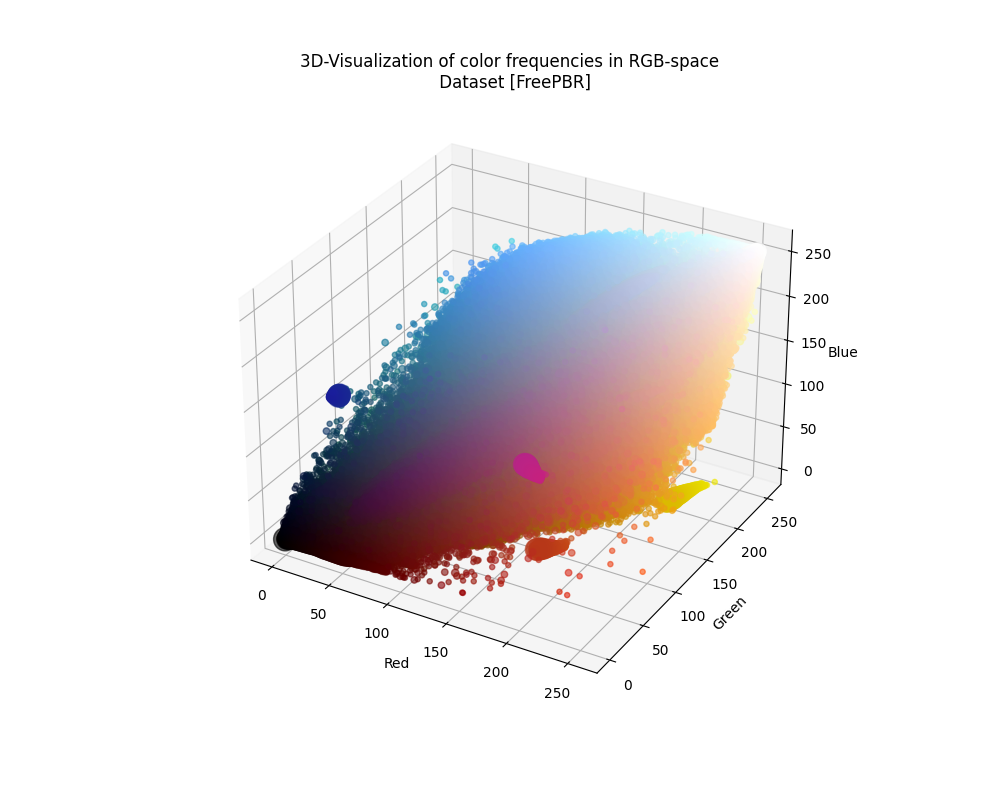
\includegraphics[width=\linewidth]{../code/dataAnalysis/output/FreePBR.png}
          \caption{FreePBR}
          \label{fig:dataset-FreePBR}
        \end{subfigure}%
        \hfill
        \begin{subfigure}{.33\textwidth}
          \centering
          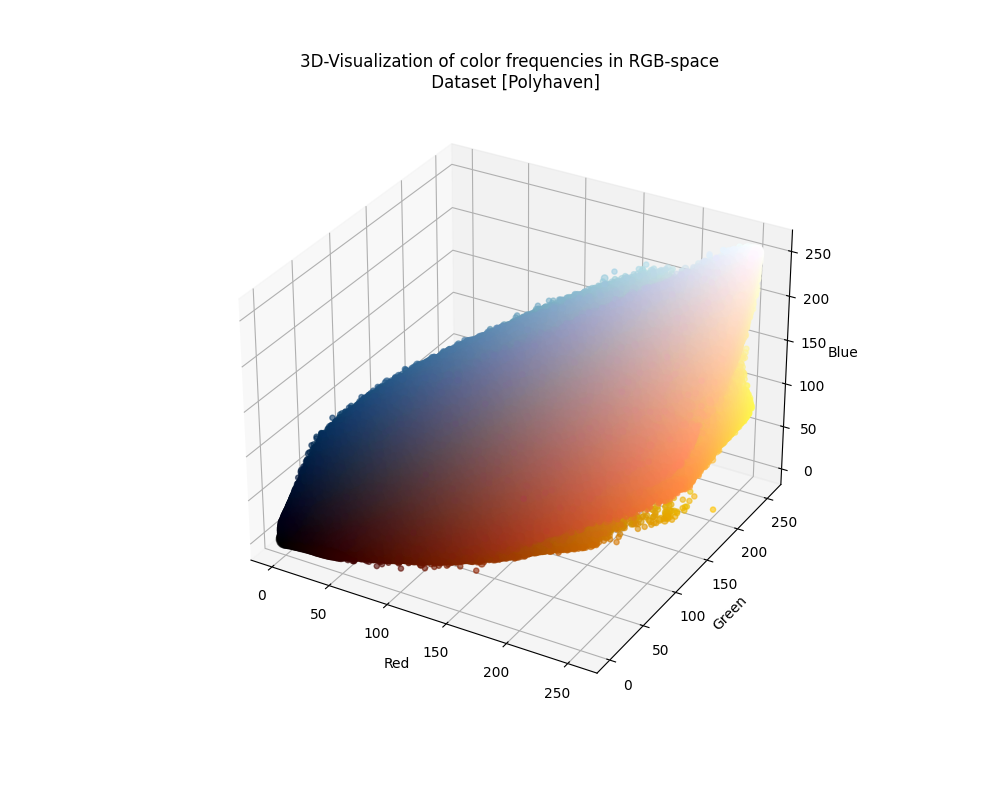
\includegraphics[width=\linewidth]{../code/dataAnalysis/output/Polyhaven.png}
          \caption{Polyhaven}
          \label{fig:dataset-Polyhaven}
        \end{subfigure}%
        \hfill
        \begin{subfigure}{.33\textwidth}
          \centering
          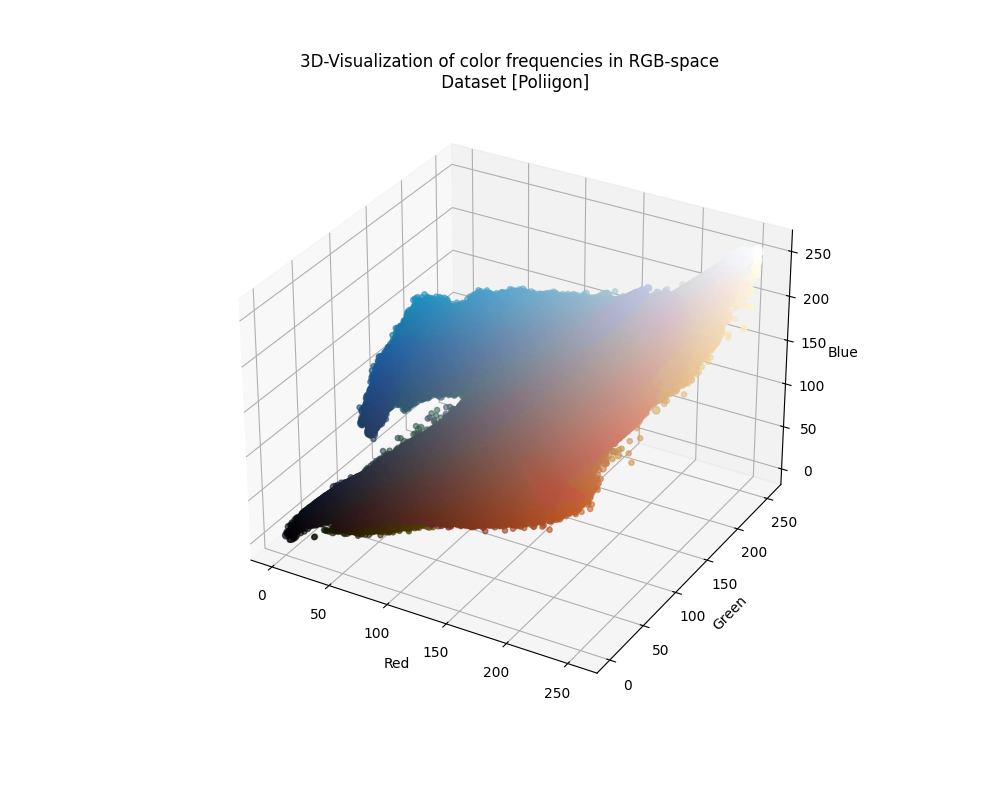
\includegraphics[width=\linewidth]{../code/dataAnalysis/output/Poliigon.png}
          \caption{Poliigon}
          \label{fig:dataset-Poliigon}
        \end{subfigure}
        
        \vspace{1cm} % Vertikaler Abstand zwischen den Reihen
        
        \begin{subfigure}{.33\textwidth}
          \centering
          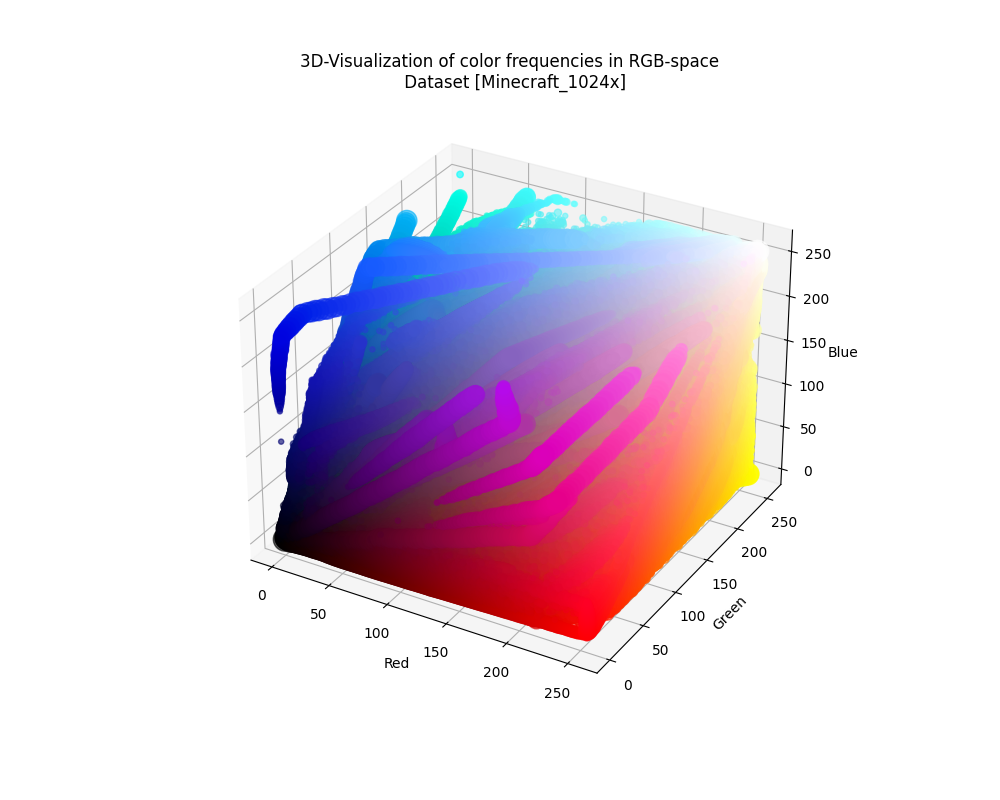
\includegraphics[width=\linewidth]{../code/dataAnalysis/output/Minecraft_1024x.png}
          \caption{Minecraft-Textures}
          \label{fig:dataset-Minecraft-Textures}
        \end{subfigure}%
        \hfill
        \begin{subfigure}{.33\textwidth}
          \centering
          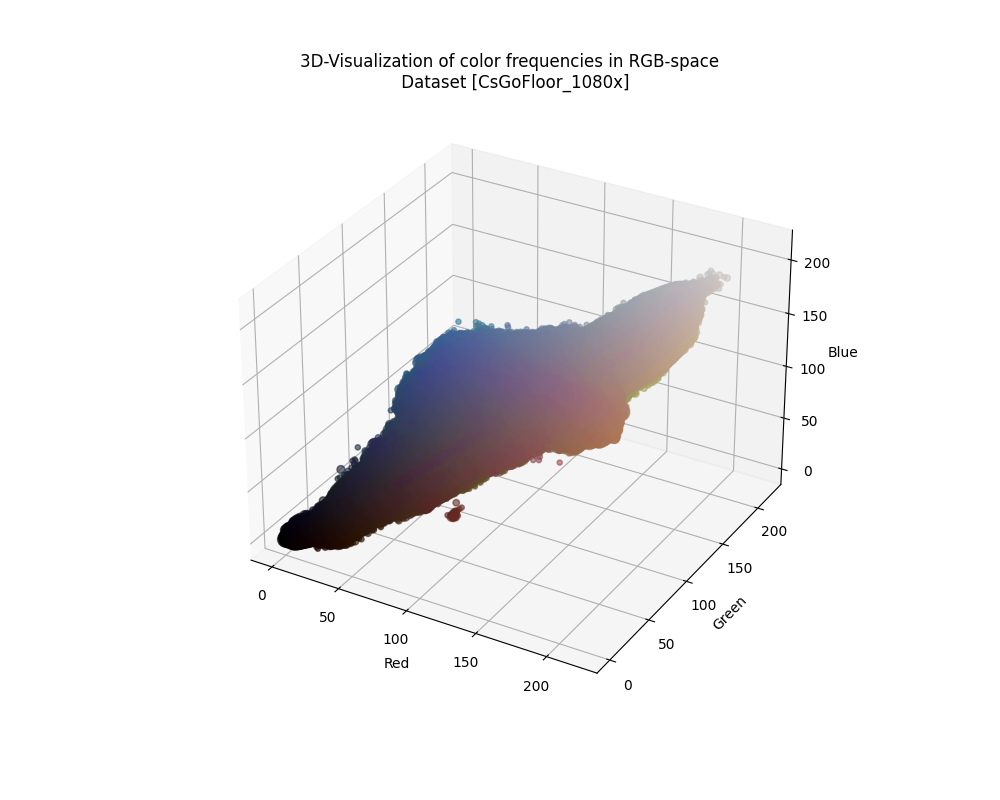
\includegraphics[width=\linewidth]{../code/dataAnalysis/output/CsGoFloor_1080x.png}
          \caption{CsGoFloor-Textures}
          \label{fig:dataset-CsGoFloor-Textures}
        \end{subfigure}%
        \hfill
        \begin{subfigure}{.33\textwidth}
            \centering
            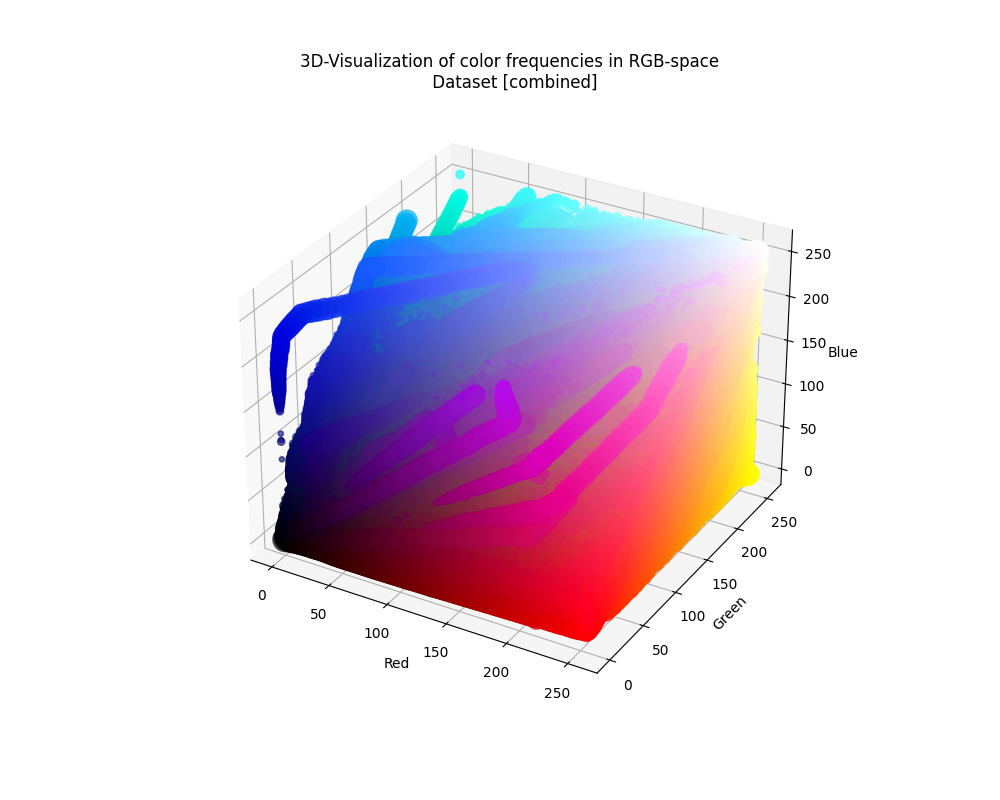
\includegraphics[width=\linewidth]{../code/dataAnalysis/output/combined.png}
            \caption{Combined}
            \label{fig:dataset-Combined}
        \end{subfigure}%
        \hfill
    \end{figure}

    In the figure above, the color distributions of the individual datasets are shown. The first five subfigures represent the color distributions of the individual datasets, while the last subfigure (\ref{fig:dataset-Combined}) shows the combined color distribution of all datasets. The color distributions of the individual datasets are quite similar, except for the Minecraft-Textures dataset, which is way more colorful than the others. The combined figure is a combination of all the individual datasets, and it is evident that the color distribution is quite diverse. This is a positive sign, as it indicates that the dataset is not focused on only a specific color spectrum.

    \subsubsection{Data Synchronization}

    In the thesis, a manual data synchronization routine is established to maintain data consistency between the supercomputer located in Berlin and the local workstation.

\subsection{Training process}
    (gpu cluster göthingen, my GPU, ...)

\subsection{Models}
    (LLMs, basic idea, roll model, spiral model) 
    \newpage

    \section{Experiment}
    
    \subsection{The Foundation of the Models}

    To build the models, a set of Python libraries is utilized, mainly PyTorch, NumPy, TensorBoard, and Einops. PyTorch serves as the core tool for constructing and training the models.
    
    The models discussed in this thesis are based on a Python script by A. Karpathy named NanoGPT \autocite{nanoGPTkarpathy2023}. This script demonstrates a straightforward and accessible GPT implementation. 
    
    \subsubsection{Data Handling}
    
    For data management, a script named dataSetCombiner is developed to load and return a combined dataset from specified image folders with optional transformations. The function combines the 33 different sources from multiple directories into a single dataset, also offering the option to apply various image transformations such as cropping, flipping, gray scaling, and color jitter.
    
    It allows for the selection between 512x512 and 1024x1024 pixel datasets, depending on the use case. Parameters can be adjusted to tailor the dataset to specific needs, such as image size, the particular dataset to load, and the option to include multiple instances of the dataset. Furthermore, it can randomly flip images vertically or horizontally to augment the dataset, thereby preventing overfitting and improving model generalization. It also supports color jittering, allowing for random adjustments in image brightness, contrast, saturation, and hue, which introduces further variability into the dataset when needed. Additionally, an option to convert images to grayscale is available.
    

\begin{figure}[H]
\centering
\begin{lstlisting}[language=Python]
    def getDataSet(path, dataset_name, size_x, size_y, repeatData=1, random_vertical_flip=False, random_horizontal_flip=False, crop_type='random', grayscale=False, color_jitter=False, jitter_brightness=0, jitter_contrast=0, jitter_saturation=0, jitter_hue=0):
\end{lstlisting}
\caption{Python function declaration: getDataSet}
\label{fig:getDataSet}
\end{figure}


    \subsubsection{Monitoring Training Progress}
    
    The training process is monitored using TensorBoard, a tool that helps visualize different aspects of training. In this thesis, TensorBoard is particularly useful for tracking training and validation loss through plots. It also allows for the viewing of the input images and the outputs generated by the models.    
    
\newpage


\subsection{Column Image Transformer}
    
    The Column Image Transformer is a transformer-based model that processes input data in a columnar format as examined in detail see \autoref{sec:IntroColumnModel}.
    
    \subsubsection{Get Data as Columns}

    The data is loaded as a DataLoader object, which is then iterated over to obtain the data in (Batch, Color, Height, Width) format. The data is then reshaped into a columnar format, resulting in a tensor of shape (Batch, Height, Color). This reshaping is achieved by indexing the data tensor as follows:

\begin{figure}[H]
\centering
\begin{lstlisting}[language=Python]

# data: (Batch, Color, Height, Width)
def get_batch(data):

    x = data[:, :BLOCK_SIZE, :BATCH_SIZE]
    y = data[:, 1:BLOCK_SIZE+1, :BATCH_SIZE]

    x = rearrange(x, 'c h b -> b h c')
    y = rearrange(y, 'c h b -> b h c')

    return x, y
\end{lstlisting}
\caption{Python function to convert data into a columnar format}
\label{fig:get_batch_CIT}
\end{figure}

    The resulting tensor \(x\) is the input to the model, and the tensor \(y\) is the target output. The \(y\) tensor is shifted by one position to the right so that the model can learn to predict the next column based on the previous columns.

    \subsubsection{Pixel Embedding}

    The input part of the data \(x\) is embedded into a higher-dimensional space using pixel embedding layers. This MLP is a straightforward linear layer that maps the input data to a higher-dimensional space, transitioning from 3 color channels to \(N_{\text{EMBD}}\). This layer consists of a linear transformation followed by a ReLU activation function and is succeeded by a dropout layer.

    Through testing and experimentation, it was discovered that the optimal configuration for the pixel embedding layer involves a specific sequence of dimensionality increases. The most effective pathway identified begins by scaling the dimensionality of the input from the original image channels \(C\) to one-fifth of \(N_{\text{EMBD}}\) (\(\frac{1}{5}N_{\text{EMBD}}\)), then increasing it to one-half of \(N_{\text{EMBD}}\) (\(\frac{1}{2}N_{\text{EMBD}}\)) until reaching \(N_{\text{EMBD}}\). The pixel embedding layer is followed by a dropout layer with a dropout rate of 0.2.

    It is crucial to highlight the importance of excluding a layer normalization (layernorm) layer in the initial few layers of the model. Incorporating layernorm early on results in outputs that are predominantly black and white. This phenomenon occurs because the color channels \(C\), which are comprised of Red, Green, and Blue, are normalized by the layernorm layer to exhibit uniform values across these channels. As a consequence, this normalization process hinders the model's ability to learn the distinct colors of the pixels, relegating it to only wrong grayscale variations.

    \subsubsection{Positional Embedding}

    \subsubsection{Classification or Regression}

    \subsubsection{Discriminator}

\newpage


\subsection{Spiral Image Transformer}
    (explanation, Data to Spiral form, positional embedding, )

    As explained in the previous section (see Section \ref{sec:IntroSpiralModel}), the spiral model is a transformer-based model that employs a spiral architecture to process input data. 

    \subsubsection{Spiral}

    To convert the 3-dimensional data (color channels, image height, image width) into a spiral form, the data must be unrolled into one dimension, resulting in an output format of (color channels, spiral length). Consequently, the data width and the height dimensions must be squeezed into a single dimension. This new form can then be utilized similarly to the data in the Column Image Transformer. As the data is flattened into a single dimension, it allows for an easy addition of positional embedding.

    \subsubsection{Spiral generation}

    The conversion of data into a spiral form needs to be highly efficient because the code block will execute for every image (batch) in the dataset. Therefore, a simple nested for loop is insufficient. In this example, fancy indexing is used to convert the data into a spiral form. Thus, the data tensor is indexed with a two-dimensional tensor containing the indices of the spiral form.

    At the start of the model training script, one indexing spiral is created to be used for all images in the dataset. The following code block illustrates the creation of the spiral index tensor.

\begin{figure}[H]
\centering
\begin{lstlisting}[language=Python]
def create_spiral(n): # n = width and height
    
    matrix = [[0] * n for _ in range(n)] # Initialize n x n matrix

    x, y = 0, 0
    # Direction vectors (right, down, left, up)
    dx = [0, 1, 0, -1]
    dy = [1, 0, -1, 0]
    direction = 0

    for i in range(n * n - 1, -1, -1):  # Start (35 for 6x6)
        matrix[x][y] = i
        nx = x + dx[direction]
        ny = y + dy[direction]

        # Change direction if the next position: out of bounds or filled
        if nx<0 or nx>=n or ny<0 or ny>=n or matrix[nx][ny]!=0:
            direction = (direction + 1) % 4  # Change direction
            nx = x + dx[direction]
            ny = y + dy[direction]

        x, y = nx, ny
    
    return torch.tensor(matrix)
\end{lstlisting}
\caption{Python function to create a spiral index tensor}
\label{fig:spiral_matrix}
\end{figure}

    The code above generates a square matrix of size n by n, then fills it with numbers in a spiral pattern, starting from the outer edge and spiraling inwards clockwise. Each cell of the matrix is assigned a unique number, beginning from the highest value in the top-left corner and decreasing by one with each step along the spiral path until reaching zero at the center or the end of the spiral. The spiral formation is achieved by moving right, then down, then left, then up, and repeating this sequence, adjusting direction whenever the next step would go out of bounds or into a cell that's already been filled.


    \subsection{Fancy Indexing into the Spiral form}

    The spiral index tensor is then used to index the data tensor, effectively converting it into a spiral form. The following image illustrates the process of converting a 7x7 image.
    
    
    \begin{figure}[H]
    \centering
    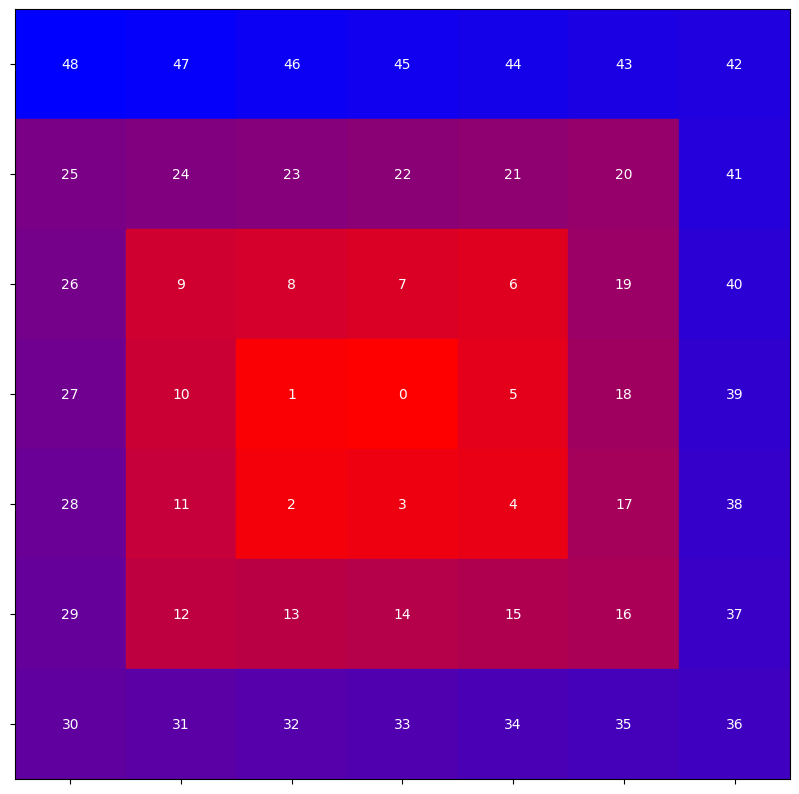
\includegraphics[width=0.6\textwidth]{../code/dataAnalysis/plots/exampleImgs/spiralShowcase1.png}
    \caption{Image representation}
    \label{fig:spiral_indexing_1}        
    \end{figure}

    \begin{figure}[H]
    \centering
    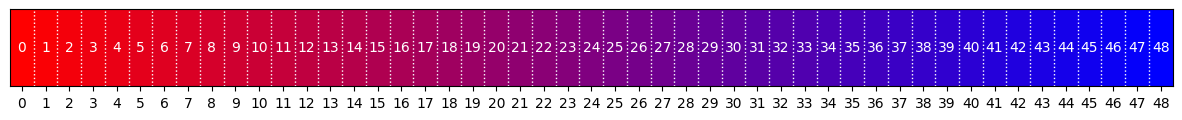
\includegraphics[width=1\textwidth]{../code/dataAnalysis/plots/exampleImgs/spiralShowcase0.png}
    \caption{7x7 Image flattened into a spiral form} 
    \label{fig:spiral_indexing_0}        
    \end{figure}

    As you can see in \autoref{fig:spiral_indexing_1}, the pixels of the image are labeled with their respective indices 0, \dots, 43. The image is then unrolled into a single dimension, as shown in \autoref{fig:spiral_indexing_0}. The centering pixel is the first element of the spiral, and the spiral continues counterclockwise from there. In the model script, the dimensions for width and height typically exceed 7, yet the underlying process remains unchanged.

\begin{figure}[H]
\centering
\begin{lstlisting}[language=Python]
  spiral_indices = torch.tensor(create_spiral(IMAGE_SIZE))

  # [...]
  # Batch_size, Color_channels, Height, Width
  B, C, H, W = data.shape

  spiral_data = torch.zeros_like(data.view(B, C, -1))

  spiral_data[:,:,spiral_indices.flatten()] = data.view(B, C, -1)

  # [...]
\end{lstlisting}
\caption{Fancy indexing to convert data into a spiral form}
\label{fig:spiral_indexing_code}
\end{figure}

    \subsubsection{Positional embedding}

\subsection{Problems}
    (layer norm(sigmoid vs clamp), color shift to gray (illustrations of average color), Text tokens vs imgs tokens)
    \newpage
    
    \section{Conclusion}\label{conclusion}  
    
This section focuses on the evaluation of the performance of the CIT and the SIT.

\subsection{Evaluation of the models}
    
    As a general conclusion it can be said that the data hints that it is possible to generate quickly new assets trow this approach. Due to the fact that the models are relatively small and the training dataset is not that big the output of the models is 

    \subsubsection{performance}
    One the big question is if it is possible to generated assets for video game. Here we can split it into two parts. The first part is to generate assets beforehand in the development cylce and in the second part is is the model so efficient that it is possible to generate assets in real time on a local machine.

    \subsubsection{quality}


\subsection{Execution locally and on the cloud}
    
    

\subsection{Further research}

    \subsubsection{LLM Scaling Laws}


    \subsection{Stable diffusion/ GANs with convolutional neural network} 
    
    

    \newpage
    \setcounter{section}{0} 
    \renewcommand*\thesection{\Alph{section}}

    \pagenumbering{roman}
    \section{Appendix}\label{appendix}
    
\subsection{Dataset Plots in the Lab Color Space}\label{sec:app_labPlots}

\begin{figure}[H]
    \centering
    \foreach \i in {-1,...,18}{
      \begin{subfigure}[t]{0.21\textwidth}
        \centering       
        \ifnum \i=-1
            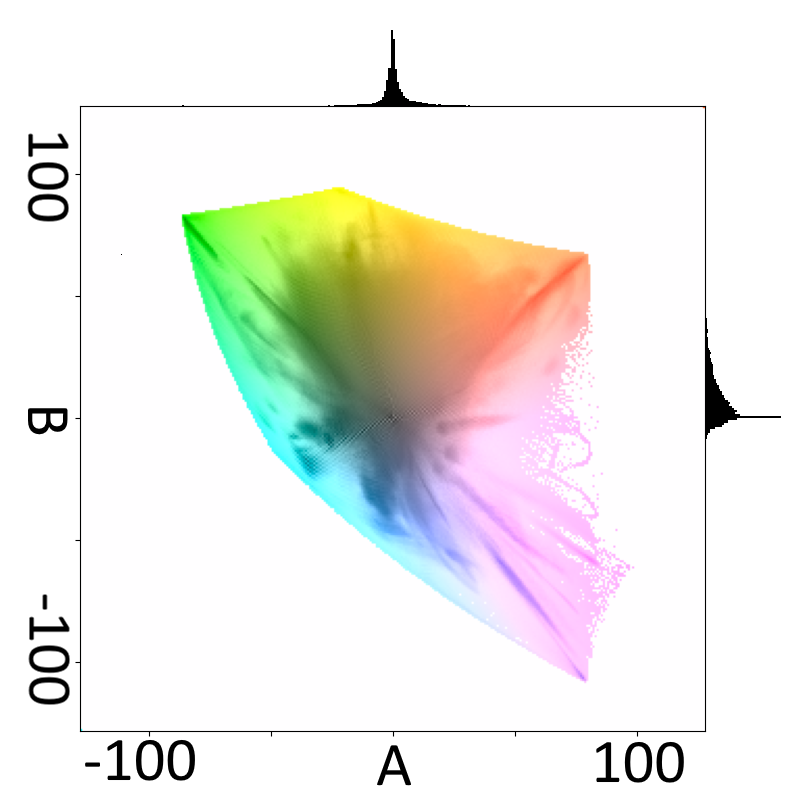
\includegraphics[width=\textwidth]{../code/dataAnalysis/plots/lab/DataCombined_lab.png}
            \caption{All Data}
        \else
            \includegraphics[width=\textwidth]{../code/dataAnalysis/plots/lab/labPlot_\i}
            \caption{source \i}
        \fi

        \label{fig:lab_sub\i}
      \end{subfigure}
      % Use the modulo operation to determine if a line break should be added
      \pgfmathparse{int(mod(\i+2,4))}
      \ifnum\pgfmathresult=0
          \newline
      \else
          \hfill
      \fi
    }
    \begin{subfigure}[t]{0.21\textwidth}
        \centering
        % No image to include, so this is left empty
        \caption*{} % Empty caption
    \end{subfigure}
    \caption*{}
    \addtocounter{figure}{-1}
\end{figure}

\begin{figure}[H]
    \centering
    \foreach \i in {19,...,33}{
      \begin{subfigure}[t]{0.21\textwidth}
        \centering       
        \ifnum \i=-1
            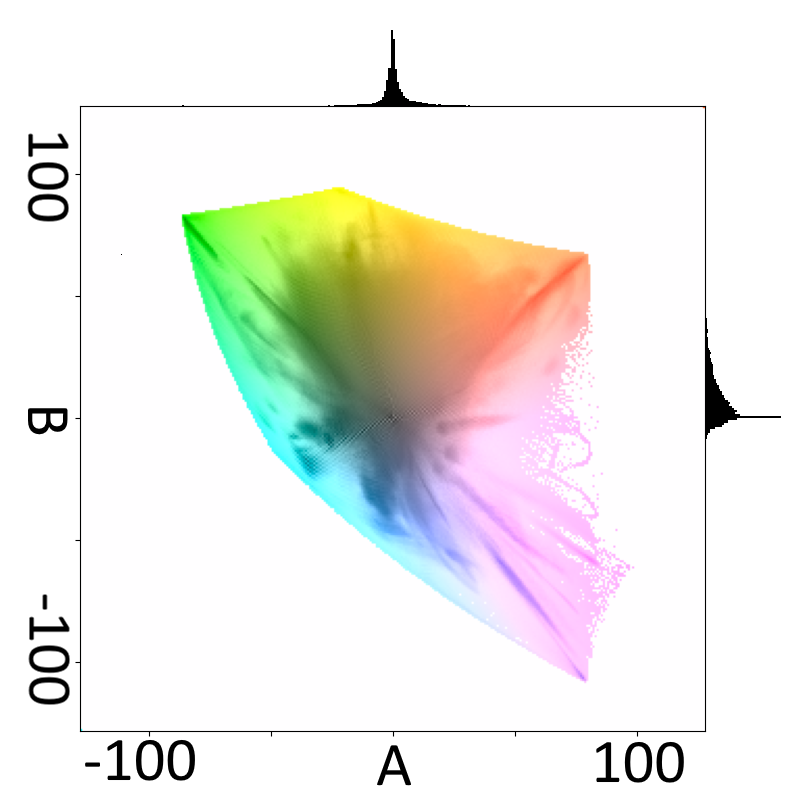
\includegraphics[width=\textwidth]{../code/dataAnalysis/plots/lab/DataCombined_lab.png}
            \caption{All Data}
        \else
            \includegraphics[width=\textwidth]{../code/dataAnalysis/plots/lab/labPlot_\i}
            \caption{source \i}
        \fi

        \label{fig:lab_sub\i}
      \end{subfigure}
      % Use the modulo operation to determine if a line break should be added
      \pgfmathparse{int(mod(\i+2,4))}
      \ifnum\pgfmathresult=0
          \newline
      \else
          \hfill
      \fi
    }
    \begin{subfigure}[t]{0.21\textwidth}
        \centering
        % No image to include, so this is left empty
        \caption*{} % Empty caption
    \end{subfigure}
    \caption{Visualization of datasets plotted in the LAB color space}
    \label{fig:lab_all2}

\end{figure}


\newpage

\subsection{Dataset Plots in the RGB Color Space}

\begin{figure}[H]
    \centering
    \foreach \i in {-1,...,18}{
      \begin{subfigure}[t]{0.21\textwidth}
        \centering

        \ifnum \i=-1
            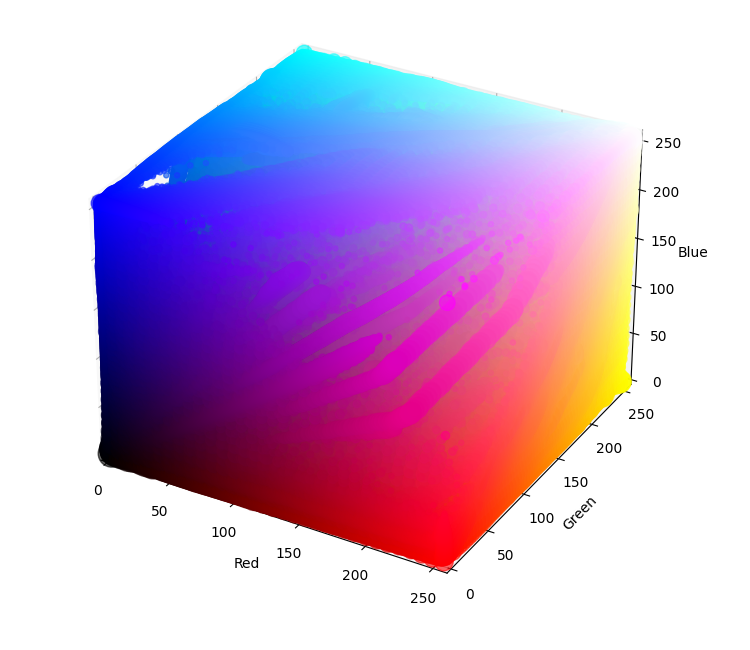
\includegraphics[width=\textwidth]{../code/dataAnalysis/plots/rgb/DataCombined_rgb.png}
        \caption{All Data}
        \else
            \includegraphics[width=\textwidth]{../code/dataAnalysis/plots/rgb/rgbPlot_\i}
            \caption{source \i}
        \fi
        \label{fig:rgb_sub\i}
      \end{subfigure}
      % Use the modulo operation to determine if a line break should be added
      \pgfmathparse{int(mod(\i+2,4))}
      \ifnum\pgfmathresult=0
          \newline
      \else
          \hfill
      \fi
    }
    \begin{subfigure}[t]{0.21\textwidth}
        \centering
        % No image to include, so this is left empty
        \caption*{} % Empty caption
    \end{subfigure}
    \caption*{}
    \addtocounter{figure}{-1}

\end{figure}

\begin{figure}[H]
    \centering
    \foreach \i in {19,...,33}{
      \begin{subfigure}[t]{0.21\textwidth}
        \centering

        \ifnum \i=-1
            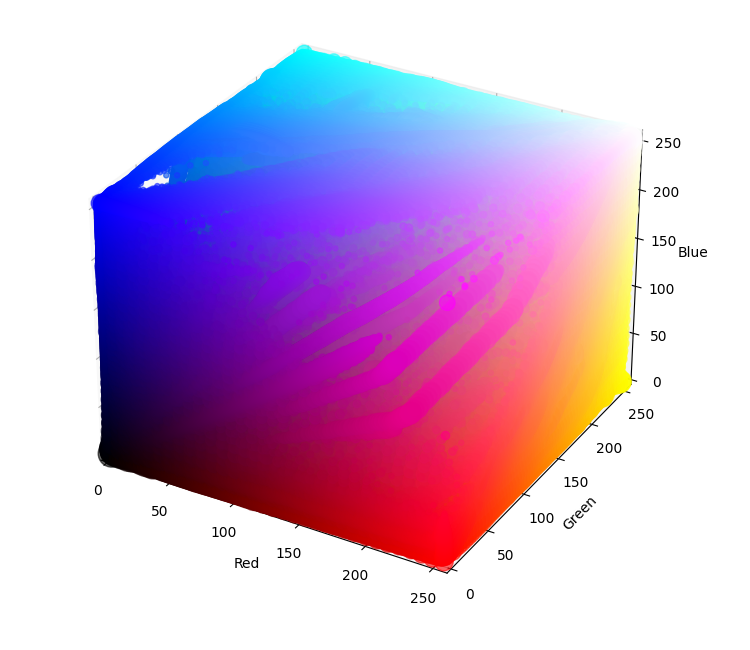
\includegraphics[width=\textwidth]{../code/dataAnalysis/plots/rgb/DataCombined_rgb.png}
        \caption{All Data}
        \else
            \includegraphics[width=\textwidth]{../code/dataAnalysis/plots/rgb/rgbPlot_\i}
            \caption{source \i}
        \fi
        \label{fig:rgb_sub\i}
      \end{subfigure}
      % Use the modulo operation to determine if a line break should be added
      \pgfmathparse{int(mod(\i+2,4))}
      \ifnum\pgfmathresult=0
          \newline
      \else
          \hfill
      \fi
    }
    \begin{subfigure}[t]{0.21\textwidth}
        \centering
        % No image to include, so this is left empty
        \caption*{} % Empty caption
    \end{subfigure}
    \caption{Visualization of datasets plotted in the RGB color space}
    \label{fig:rgb_all}

\end{figure}

\newpage
\begin{landscape}
\subsection{Trained Models with hyperparameters}
\label{sec:trained_models_hyperparameters}


\begin{table}[H]
    \centering
    \begin{threeparttable}
    \caption{Model Configuration Overview}
    \scriptsize
    \begin{tabular}{|c|c|c|c|c|c|c|c|c|c|c|c|c|}
    \toprule
    MODEL & Nr. & VER. & BATCH\_SIZE & BLOCK\_SIZE & N\_EMBD & N\_HEAD & N\_LAYER & PARAMETER\tnote{*} & GPUS & DATASET & VAL\_LOSS\tnote{**}  \\
    \midrule
    \multirow{5}{*}{\rotatebox{90}{CIT}}
    & 0 & 2.1.7.0 & 128 & 128 & 128 & 6 & 6 & 1.22 m & 1 & old Dataset & 0.0082  \\
    & 1 & 2.1.8.0 & 64 & 64 & 128 & 6 & 6 & 1.21 m & 1 & x512 Dataset & 0.0035 \\
    & 2 & 2.1.8.0 Classify & 64 & 64 & 128 & 6 & 6 & 1.25 m & 1 & x512 Dataset & 1.841 \\
    & 3 & 2.1.8.0 & 64 & 256 & 512 & 8 & 8 & 25.66 m & 4 & x512 Dataset & 0.0025 \\
    & 4 & 2.1.8.0 & 32 & 511 & 640 & 9 & 9 & 45.09 m & 4 & x512 Dataset & 0.0024 \\
    \midrule
    \multirow{2}{*}{\rotatebox{90}{SIT}}
    & 5 & 5.0.1.0 & 8 & 4,095 & 128 & 6 & 6 & 1.73 m & 1 & x512 Dataset & 0.0074 \\
    & 6 & 5.0.1.0 & 4 & 4,095 & 512 & 8 & 8 & 27.62 m & 1 & x512 Dataset & 0.0027 \\
    \bottomrule
    \end{tabular}
    \begin{tablenotes}
    \item[*] Figures in millions
    \item[**] Average of the last 5 validation loss values
    \end{tablenotes}
    \end{threeparttable}
\end{table}

\end{landscape}

\newpage

\subsection{Local workstation setup}

\begin{table}[H]
    \centering
    \begin{tabularx}{0.90\textwidth}{|X|X|}
    \hline
    \textbf{Component} & \textbf{Specification} \\ \hline
    Operating System & Microsoft Windows 11 Pro \\ \hline
    CPU & AMD Ryzen 9 7900X 12 cores, 4.7 GHz \\ \hline
    GPU & NVIDIA RTX 3090 \\ \hline
    RAM & 64 GB (DDR5-6000) \\ \hline
    SSD & 2TB Samsung 990 PRO M.2 PCIe 4.0 \\ \hline
    \end{tabularx}
    \caption{Local workstation setup}
    \label{table:workstation_setup}
\end{table}
    
\begin{table}[H]
    \centering
    \begin{tabularx}{0.90\textwidth}{|X|X|}
    \hline
    \textbf{Component} & \textbf{Specification} \\ \hline
    CPU & 2x Intel Xeon "Ice Lake" Platinum 8360Y (36 cores per socket, 2.4 GHz) \\ \hline
    GPU & 4x Nvidia A100 (80GB HBM2, SXM) \\ \hline
    RAM & 1 TB RAM (DDR4-3200) \\ \hline
    SSD & 7.68 TB NVMe local SSD \\ \hline
    \end{tabularx}
    \caption{Single slurm compute node}
    \label{table:server_setup}
\end{table}

\newpage

\subsection{Transformer layer implementation}
\label{sec:transformer_layer_Python}

\begin{lstlisting}[language=Python]
class Head(nn.Module):
""" one head of self-attention """

    def __init__(self, head_size):
        super().__init__()
        self.key = nn.Linear(N_EMBD, head_size, bias=False)
        self.query = nn.Linear(N_EMBD, head_size, bias=False)
        self.value = nn.Linear(N_EMBD, head_size, bias=False)
        self.register_buffer('tril', torch.tril(torch.ones(BLOCK_SIZE, BLOCK_SIZE)))

        self.dropout = nn.Dropout(DROPOUT)

    def forward(self, x):
        # input of size (batch, time-step, channels)
        # output of size (batch, time-step, head size)
        B,T,C = x.shape
        k = self.key(x)   # (B,T,hs)
        q = self.query(x) # (B,T,hs)
        # compute attention scores ("affinities")
        wei = q @ k.transpose(-2,-1) * k.shape[-1]**-0.5 # (B, T, hs) @ (B, hs, T) -> (B, T, T)
        wei = wei.masked_fill(self.tril[:T, :T] == 0, float('-inf')) # (B, T, T)
        wei = F.softmax(wei, dim=-1) # (B, T, T)
        wei = self.dropout(wei)
        # perform the weighted aggregation of the values
        v = self.value(x) # (B,T,hs)
        out = wei @ v # (B, T, T) @ (B, T, hs) -> (B, T, hs)
        return out

class MultiHeadAttention(nn.Module):
""" multiple heads of self-attention in parallel """

    def __init__(self, num_heads, head_size):
        super().__init__()
        self.heads = nn.ModuleList([Head(head_size) for _ in range(num_heads)])
        self.proj = nn.Linear(head_size * num_heads, N_EMBD)
        self.dropout = nn.Dropout(DROPOUT)

    def forward(self, x):
        out = torch.cat([h(x) for h in self.heads], dim=-1)
        out = self.dropout(self.proj(out))
        return out

class FeedFoward(nn.Module):
""" a simple linear layer followed by a non-linearity """

    def __init__(self, n_embd):
        super().__init__()
        self.net = nn.Sequential(
            nn.Linear(n_embd, 4 * n_embd),
            nn.ReLU(),
            nn.Linear(4 * n_embd, n_embd),
            nn.Dropout(DROPOUT),
        )

    def forward(self, x):
        return self.net(x)

class Block(nn.Module):
""" Transformer block: communication followed by computation """

    def __init__(self, n_embd, n_head):
        # n_embd: embedding dimension, n_head: the number of heads we'd like
        super().__init__()
        head_size = n_embd // n_head
        self.sa = MultiHeadAttention(n_head, head_size)
        self.ffwd = FeedFoward(n_embd)
        self.ln1 = nn.LayerNorm(n_embd)
        self.ln2 = nn.LayerNorm(n_embd)

    def forward(self, x):
        x = x + self.sa(self.ln1(x))
        x = x + self.ffwd(self.ln2(x))
        return x
\end{lstlisting}

This code snippet shows the implementation of the transformer layer in the Column Image Transformer and the Spiral Image Transformer. The code above is heavily inspired by the implementation of the script by A.
Karpathy named NanoGPT \autocite{nanoGPTkarpathy2023} \autocite{nanogpt-lecturekarpathy2023}



    \newpage
        
    \pagestyle{empty}
    \pagenumbering{gobble}
    \section{Eidesstattliche Erklärung}
    
    Ich versichere, die von mir vorgelegte Arbeit selbständig verfasst zu haben.
    Alle Stellen, die wörtlich oder sinngemäß aus veröffentlichten oder nicht veröffentlichten Arbeiten anderer entnommen sind,
    habe ich als entnommen kenntlich gemacht.\\ 
    Sämtliche Quellen und Hilfsmittel, die ich für die Arbeit benutzt habe, sind
    angegeben. Die Arbeit hat mit gleichem Inhalt bzw. in wesentlichen Teilen noch keiner anderen Prüfungsbehörde vorgelegen.\\\\
    \begin{tabular}{cp{7cm}}
    & \\ 
    & \\ \hline
    \small (Ort, Datum, Unterschrift) & \normalsize \\
    \end{tabular}
    
    
    \newpage
    \printbibliography

    \thispagestyle{empty}
    \newpage

\end{document}

